\documentclass[tikz,border=2pt]{standalone}
\usepackage[T1]{fontenc}\usepackage{helvet}\renewcommand{\familydefault}{\sfdefault}
\usetikzlibrary{arrows.meta,positioning,fit,backgrounds,calc}
\begin{document}
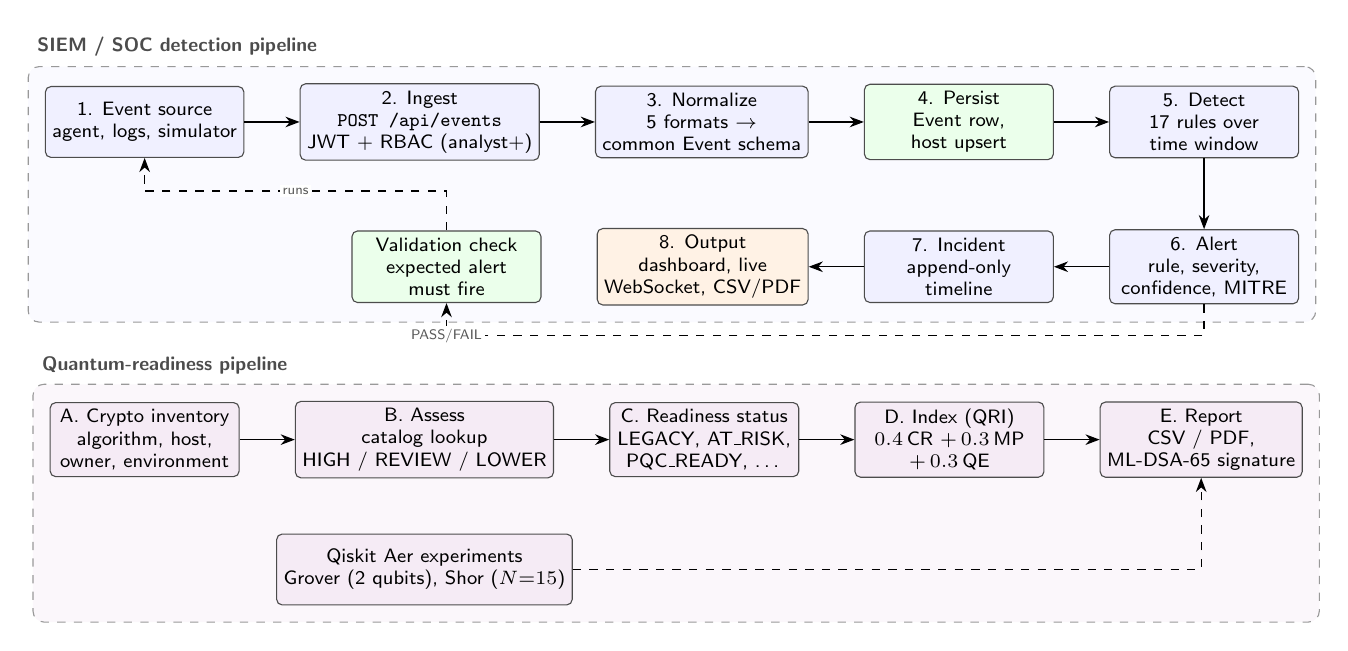
\begin{tikzpicture}[font=\scriptsize,
 box/.style={draw=black!70,rounded corners=2pt,fill=white,align=center,minimum height=9mm,minimum width=24mm,inner sep=2.5pt,line width=0.4pt},
 sbox/.style={box,fill=blue!6},qbox/.style={box,fill=violet!8},dbox/.style={box,fill=green!8},obox/.style={box,fill=orange!10},
 lab/.style={font=\scriptsize\bfseries,text=black!70},
 ar/.style={-{Stealth[length=1.8mm]},line width=0.45pt},
 ln/.style={font=\tiny,text=black!65,midway,fill=white,inner sep=1pt}]
% SIEM lane
\node[sbox] (src) {1. Event source\\agent, logs, simulator};
\node[sbox,right=7mm of src] (api) {2. Ingest\\\texttt{POST /api/events}\\JWT + RBAC (analyst+)};
\node[sbox,right=7mm of api] (norm) {3. Normalize\\5 formats $\rightarrow$\\common Event schema};
\node[dbox,right=7mm of norm] (ev) {4. Persist\\Event row,\\host upsert};
\node[sbox,right=7mm of ev] (det) {5. Detect\\17 rules over\\time window};
\node[sbox,below=9mm of det] (al) {6. Alert\\rule, severity,\\confidence, MITRE};
\node[sbox,left=7mm of al] (inc) {7. Incident\\append-only\\timeline};
\node[obox,left=7mm of inc] (ui) {8. Output\\dashboard, live\\WebSocket, CSV/PDF};
\node[dbox,left=7mm of ui] (val) {Validation check\\expected alert\\must fire};
\draw[ar] (src)--(api); \draw[ar] (api)--(norm); \draw[ar] (norm)--(ev); \draw[ar] (ev)--(det);
\draw[ar] (det)--(al); \draw[ar] (al)--(inc); \draw[ar] (inc)--(ui);
\draw[ar,dashed] (al.south) -- ++(0,-4mm) -| node[ln,pos=0.5]{PASS/FAIL} (val.south);
\draw[ar,dashed] (val.north) -- ++(0,5mm) -| node[ln,pos=0.25]{runs} (src.south);
\node[font=\tiny,text=black!65,below=1mm of val] {};
% Quantum lane
\node[qbox,below=31mm of src] (inv) {A. Crypto inventory\\algorithm, host,\\owner, environment};
\node[qbox,right=7mm of inv] (as) {B. Assess\\catalog lookup\\HIGH / REVIEW / LOWER};
\node[qbox,right=7mm of as] (rd) {C. Readiness status\\LEGACY, AT\_RISK,\\PQC\_READY, \dots};
\node[qbox,right=7mm of rd] (qri) {D. Index (QRI)\\$0.4\,$CR $+\,0.3\,$MP\\$+\,0.3\,$QE};
\node[qbox,right=7mm of qri] (rep) {E. Report\\CSV / PDF,\\ML-DSA-65 signature};
\node[qbox,below=7mm of as] (qk) {Qiskit Aer experiments\\Grover (2 qubits), Shor ($N{=}15$)};
\draw[ar] (inv)--(as); \draw[ar] (as)--(rd); \draw[ar] (rd)--(qri); \draw[ar] (qri)--(rep);
\draw[ar,dashed] (qk.east) -| (rep.south);
\begin{scope}[on background layer]
 \node[draw=black!40,dashed,rounded corners=4pt,fill=blue!2,inner sep=6pt,fit=(src)(api)(norm)(ev)(det)(al)(inc)(ui)(val),label={[lab,anchor=south west]north west:SIEM / SOC detection pipeline}] {};
 \node[draw=black!40,dashed,rounded corners=4pt,fill=violet!3,inner sep=6pt,fit=(inv)(as)(rd)(qri)(rep)(qk),label={[lab,anchor=south west]north west:Quantum-readiness pipeline}] {};
\end{scope}
\end{tikzpicture}
\end{document}
